\section{Experiment}
\label{sec:experiment}
% a simple tool for multiple choice dataset evaluation and correction

We proceed to demonstrate the effectiveness of our framework in three aspects:
First, we use our method to detect cues and measure the amount of information leak
in 12 datasets from 6 different tasks, as shown in~\tabref{tab:datasets_exp}. 
Second, we evaluate the true reasoning power of a number of popular NLP
models on original test sets that are split into 
easy and hard part. 
Third, we attempt to improve the models performance by training on the filtered
version of the training data.
%\KZ{Give a table of the basic stats of these datasets? Why 1 less than yesterday?
%Also give the models for each the datasets in another table to give ppl a birds eyes view.} 
 
 %\end{itemize}

\begin{table*}[th]
\centering
\includegraphics[width=2\columnwidth]{picture/datasets_exp.eps}
\caption{Data examples and normalized version.}
\label{tab:datasets_exp}
\end{table*}

 \subsection{Our Results on Different Tasks}
 \label{sec:experiment1}
 
 We experiment on 12 datasets in \tabref{tab:datasets_exp}. 
 %These datasets are widely used in their 
 %respective fields to provide relevant knowledge and evaluate whether 
% models have the ability to solve the the problems in a field. %
%We have give some examples in \figref{fig:datasets_exp}. 
These datasets can mainly be classified into two types of tasks. 
The first type are the NLI classification tasks, a special case of multiple choice datasets. 
The second type are the multiple choice problems, including ARCT, 
ARCT\_adv\cite{schuster2019towards}, 
RACE~\cite{lai2017race}, and RECLOR~\cite{yu2020reclor}, in which ``hypothesis'' 
is one of the alternatives and ``premise'' contains more than one context roles. 
%\KZ{Don't understand: only has the premise and the hypothesis without the choices.}
For example, in~\tabref{tab:datasets_exp}, 
ARCT dataset have \textbf{Reason} and \textbf{Claim} as ``premise'' 
which requires to select the right warrant between them. 
%The alternative warrant is the hypothesis and the premise is consist of  reason and claim. 
%RACE and Reclor includes context and questions which will be seen as ``premise''. 
%The label for each alternative is 
%``true'' or ``false'' for whether this hypothesis is the correct one.
Ubuntu~\cite{lowe2015ubuntu}, COPA~\cite{roemmele2011choice}, ROCStory, SWAG~\cite{zellers2018swag} and 
CQA~\cite{talmor2019commonsenseqa} also belong to the second type but with only context role 
in ``premise''.
Moreover, In \tabref{dataset_intro}, we 
show how the hypotheses are collected in these datasets. The hypothesis 
in most of datasets are written by human, except for CQA and SWAG. And only two of
them have adversarial experiments to amend the datasets.    
 
\begin{table}[h]
\small
\centering
\begin{tabular}{p{7mm}cccccc}\hline
\textbf{Datasets} &Data Size & Data source& AE& Human(\%)\\ \hline                                   
ROCStory & 3.9k         & CD         &No    &100.0  \\
COPA        & 1k           &  CD           &No   &100.0     \\
SWAG       & 113k       &  LM            &Yes  & 88.0\\
SNLI          &  570K     & CD           &No     &80.0\\
QNLI         & 11k         &  CD            &No    &80.0\\
MNLI         & 413k       &  CD            & No   &80.0\\
RACE        & 100k      &  CD            &No    &94.5\\
RECLOR       &  6k          &  CD             &No   &63.0\\
CQA         & 12k        &  CD              &No    &88.9\\
ARCT         & 2k         & CD               &No    &79.8\\
ARCT\_adv& 4k         & CD                &Yes   & -\\
Ubuntu   & 100k      &Random Selection & No  & -  \\
\hline
\end{tabular}
\caption{\label{dataset_intro} The methods of hypothesis collection for
the datasets.  
AE = Adversarial Experiment, LM = language model, CD = crowdsourcing, Human represents 
human performance on the datasets.}
\end{table}
 
To show if the word cues really exist in these datasets, 
we use diverse metrics (in~\secref{sec:approach}) to get cue features. 
Then we use four simplest ways, the average value classifier (Ave), 
the maximum value classifier (Max), SGD classifier (SGDC) and 
logistic regression (LR) (\secref{sec:approach}), 
to make decision using only the spurious statistical cues. 

In order to measure the severity of information leak in data sets, we propose to 
In order to measure the severity of information leak in data sets, we propose to 
use the deviation of accuracy from the majority prediction as a measurement which can be expressed as:
\begin{equation}
    \mathcal{D} = {Acc} - {Majority}
\end{equation}

${Majority}$ is the accuracy with majority voting. When the label distribution is balanced, the majority 
voting is equal to random selection. ${Acc}$ represents the prediction result of 
a model based on spurious cues only. 
The difference between our method and the hypothesis-only method (which serves as
the gold standard here) is that our method uses word-level cues that are interpretable,
whereas the hypothesis-only method uses more complex cues extracted by advanced models
which is not interpretable.

\tabref{tab:hate} reports a cue
(the word ``hate'') that is overwhelmingly found in the negative
endings. This similarity imbalanced distribution between train and test dataset is ``leakage''.
Obviously, the higher absolute value of $\mathcal{D}$ suggests 
the existence of larger amount of cues in a dataset. The opposite, that is, 
smaller $\mathcal{D}$ doesn't mean bias in the training data is small, 
but less ``leakage'' between the training and test data. 
That is, the biases can be different between training and testing dataset.
If $\mathcal{D}$ is positive, it means the 
model takes advantage of the cues in its prediction.
%Otherwise, it indicates that the dataset is harder with
%inconsistent statistical cues.  
This evaluation method is general and can be used on any multiple choice dataset. 
%For providing  a high quality stress test dataset, 
%the first condition is that it's hard to 
%choose right choice with ``leakage'' feature only. In another word, 
%it's important to break the ``leakage'' between them.

\begin{table}[th]
\small
\centering
\begin{tabular}{lccc}
\hline
\textbf{Dataset}& Pos ending& Neg ending &Total\\
\hline
Training set & 3  & 70 &73\\
Test set          & 4  & 69 &73\\
\hline
\end{tabular}
\caption{Frequency of word ``hate'' appearing in the positive and 
negative endings of ROCStories training and test datasets.}
\label{tab:hate}
\end{table}

%\begin{table*}[th]
% \scriptsize
%\centering
%\begin{tabular}{p{10mm}cccc|cccc|cccc}\hline
%\textbf{Datasets} & \multicolumn{4}{c|}{Top1} & \multicolumn{4}{c|}{Top2} &  \multicolumn{4}{c}{Top3} \\ \hline
%                           & \multicolumn{2}{c}{Unigram} &  \multicolumn{2}{c|}{Cross-unigram}&  \multicolumn{2}{c}{Unigram} &  %\multicolumn{2}{c|}{Cross-unigram}& \multicolumn{2}{c}{Unigram} &  \multicolumn{2}{c}{Cross-unigram}\\ \hline   
%                           &Metric &Method  &Metric &Method &Metric &Method &Metric &Method &Metric &Method &Metric %&Method \\ \hline    
%ROCStory  &RF&LR & CP&LR     &    CP&LR &RF&LR      &RF&SGDC&PMI&LR\\
%SNLI          &PMI&LR& PMI&LR   &    CP&LR  &CP&LR     &CP&SGDC&RF&LR\\
%QNLI         &Freq&LR& CP&LR    &    CP&LR  & CP&AveC           &PMI&LR  &PMI&AveC \\
%MNLI         &CP&LR  &CP&LR     &     PMI&LR & CP&SGDC         &CP&SGDC &RF&LR\\
%RACE        & CP&LR &CP&LR     &    CP&SGDC & PMI&LR          &PMI&LR& RF&LR\\
%RECLOR      & Cos&LR &CP&LR     &   Cos&SGDC  & RF&LR      &CP&LR&  Cos&LR\\
%\hline
%\end{tabular}
%\caption{\label{best_method} Top three corresponding metrics and 4 simple classification methods of accuracy ranking on different datasets.}
%\end{table*}

\begin{table*}[th]
\small
\centering
\begin{tabular}{ccccccccccccc}
\hline
     & \multicolumn{3}{c}{Ave}      & \multicolumn{3}{c}{Max}      & \multicolumn{3}{c}{SGDC}       & \multicolumn{3}{c}{LR}     \\ \hline
     & fastText & BERT & P     & fastText & BERT & P     & fastText & BERT & P     & fastText & BERT & P     \\ \hline
PMI  & 90.87       & 96.23   & 93.55 & 95.37       & 79.82   & 87.59 & 97.81       & 91.01   & 94.41 & 97.14       & 96.05   & 96.6  \\
LMI  & 65.13       & 49.18   & 57.16 & 34.52       & 30.71   & 32.62 & 69.88       & 79.06   & 74.47 & 77.46       & 81.21   & 79.33 \\
AD   & 84.62       & 72.49   & 78.56 & 90.75       & 73.02   & 81.89 & 93.73       & 76.24   & 84.98 & 97.56       & 86.91   & 92.24 \\
WP   & 86.87       & 73.09   & 79.98 & 92.47       & 79.87   & 86.17 & -3.1        & 22.59   & 9.74  & 56.16       & 75.55   & 65.86 \\
RD   & 96.59       & 93.82   & 95.21 & 98.23       & 91.04   & 94.63 & 94.30       & 93.98   & 94.14 & 94.21       & 95.59   & 94.90 \\
Cos  & 94.84       & 82.94   & 88.89 & 92.73       & 75.40   & 84.07 & 98.08       & 87.86   & 92.97 & 87.38       & 78.44   & 82.91 \\
Freq & 68.00       & 50.02   & 59.01 & 34.45       & 30.67   & 32.56 & 64.08       & 67.11   & 65.60 & 74.58       & 88.64   & 81.61 \\
CP   & 93.09       & 96.61   & 94.85 & 95.29       & 79.80   & 87.54 & 97.19       & 96.16   & 96.67 & 97.17       & 97.34   & \textbf{97.26} \\ \hline
\end{tabular}
\caption{\label{best_method} The Pearson Score of $\mathcal{D}$ on 12 datasets, between our methods and hypothesis-only models, fastText and BERT. 
P is the average Pearson score of BERT and fastText.}
%with word cue features on sixP\_BERT data sets. It's the number and proportion of accuracy ranking in the top three (the max number must be six because there are only six data sets)
\end{table*}



To track the deviation performance $\mathcal{D}$ of hypothesis-only models,
we use Pearson Correlation Coefficient(PCC) score to estimate the correlation 
of deviation results between our methods and hypothesis-only models.  
We used all the combinations of 8 cue score metrics and 
4 aggregation algorithms on 12 datasets. We get the 12 deviations of each methods,
one for each dataset. 
Meanwhile, we get hypothesis-only deviation results of fasttext and BERT. 
%Then we calculate all Pearson score between each of our method and hypothesis-only 
%results. 
The correlation result is shown in~\tabref{best_method}. 
We can find that CP cue score with logistic regression model scores 97.17\% 
with fastText and 97.34\% with BERT which indicates its high correlation 
with the golden standard hypothesis-only models. 
Thus we choose CP with logistic regression method to evaluate all datasets in
the remaining experiments. 
To further illustrate this trend, we plot $\mathcal{D}$ for 
our CP+LR method and 2 hypothesis-only models (fastText and BERT) on 12 datasets
in \figref{fig:d_figure}. 
We can clearly see that the lines are tracking very closely.

\begin{figure}[th]
\centering
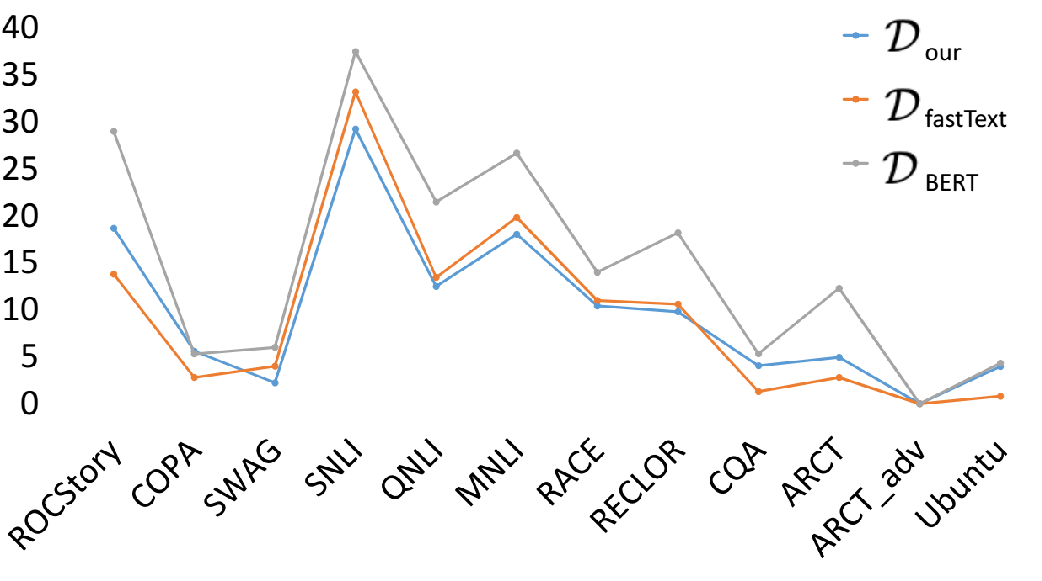
\includegraphics[width=1.0\columnwidth]{picture/d_figure.pdf}
\caption{Deviation scores for three prediction models on all 12 datasets.}
\label{fig:d_figure}
\end{figure}


In \tabref{best_acc}, the selection
%\KZ{Don't use such emotional terms: absurd} 
results through word cue features on several datasets are striking.
For example the highest accuracy with our methods for ROCStories dataset 
substantially exceeds the random selection probability by 20.92\% and even higher  for SNLI dataset 
by 33.59\%.  As was expected, 
manually intervened datasets without adversarial experiment 
for filtering contain more spurious statistical cues. 
The result for ARCT\_adv which adjust ARCT dataset by human does have a certain effect (from 54.95\% to 50\%).
But how deviation $\mathcal{D}$ identifies which datasets are seriously problematic? 
Based on our experience, if $\mathcal{D}$ of a models beyond 10\% on either cue feature, this model will be 
determined as a problematic dataset.
%statistical cues problem.we define the boundaries 
%for this purpose on 10\%. 
%We train fastText and BERT model with hypothesis-only and test on 12 datasets except for CQA, 
%since CQA only take toks 
%The results are shown in~\figref{}. 
%consider 
ROCStories, SNLI, MNLI, QNLI, RACE and RECLOR are the datasets containing heavier
statistical cue problem. 6 out of 12 datasets are ``bad'' datasets which 
indicates word 
cues are general problems for multiple choice datasets. 

\begin{table}[th]
\small
\centering
\begin{tabular}{lcccccc}\hline
\textbf{Datasets} &Majority & \multicolumn{2}{c}{Word Cues}  \\ \hline
                                     & (\%)                 &  Acc.(\%) & $\mathcal{D}(\%)$ \\ \hline         
ROCStory & 50.0            & 68.68          & \textbf{18.68}   \\
COPA        & 50.0           & 55.60           &  5.60                \\
SWAG       & 25.0           & 27.23           &   2.23                \\
SNLI          & 33.33      & 62.57           &  \textbf{29.24}      \\
QNLI         & 50.0           & 62.49            &  \textbf{12.49}   \\
MNLI         & 33.33      & 51.37            &\textbf{18.04}        \\
RACE        & 25.0          & 35.42            &   \textbf{10.42}   \\
RECLOR       & 25.0           & 34.80            &   9.80   \\
CQA          &20.0            & 23.42            &  3.42      \\
ARCT        & 50.0            & 54.95           &  4.95      \\
ARCT\_adv& 50.0           &50                 &0.0      \\
Ubuntu   & 1.0               &4.96              &3.96      \\
\hline
\end{tabular}
\caption{\label{best_acc} Highest accuracy of our 4 simple classification models
on 12 datasets and the deviations from majority selection.}
\end{table}

 %%There is an another way to determine which cue metric can better represent cue features 
 %and which method is proper to aggregate the cue features 
 %for exploring the weaknesses in the datasets. We have 8 cue metrics and 4 aggregation 
 %methods to select the choices. Trying on all permutation, we can choose the 
 %best one which can get high accuracy all the time. 
 %The number of the combination cue metrics and methods that can get the accuracy is shown in~\tabref{best_method2} (detailed scores for all permutation are recorded
%in Appendix).
 %, top three corresponding metrics and classification methods of accuracy ranking on problematic 
 %datasets we mentioned above. in~\tabref{best_method}, 
 %By observing the results,
 %It is apparent that  the conditional probability(CP) with logistic regression(LR) is 
 %most likely to fully utilize cues for getting the best results. Meanwhile, 
 %CP, Freq, PMI, RF and Cos are better to measure the degree of word cues then LMI 
 %and WP which also consider the term frequency. It indicates that the low frequency but 
 %highly unbalanced tokens can also influence the decision heavily. 
 %We can deem that cue features has relatively small 
 %relationship with frequency. It is noted that we will only use CP metric and LR 
 %method to get spurious feature and split datasets.
 
%\begin{table}[th]
%\scriptsize
%\centering
%\begin{tabular}{p{7mm}ccccc}
%\hline
%Method & Metric & \multicolumn{2}{c}{Word Cues}\\ \hline    
%            &              & Num. & \%\\ \hline    
%LR&CP&  6 & 100\\
%LR&PMI  &4&66.67\\
%LR&RF&  1 &  16.67\\
%SGDC&CP&3&50.0\\
%LR&Freq &1&16.67\\
%LR&Cos  & 1&16.67\\
%SGDC&RF&1&16.67\\
%SGDC&Cos&1&16.67\\
%\hline    
%\end{tabular}
%\caption{\label{best_method2} Test cue metrics and aggregation methods with word cue features on six data sets. It's the number and proportion of accuracy ranking in the top three (the max number must be six because there are only six data sets)}
%\end{table}

 We have shown to what extent a dataset 
 contains word cues by deviation $\mathcal{D}$. The original datasets are 
 automatically be separated into easy and hard part that is determined by whether the instance 
 can be correct chosen or not.
 Moreover, it is suspicious that whether the models really learn these features 
 to make good performance or not. We will explore more in the following sections.
 
 
\subsection{Performance Gap on Easy and Hard Part}
\label{sec:experiment2}
%\KZ{Instead of deviation, call it ``performance gap''?}
If a model learns the cue features in a dataset, It 
 will probably make a tendentious choice on 
 test set according to the samples whether have same cue features or not. 
 Thus we make an assumption that if a model is affected by cues 
in the dataset, it will have different performance on easy and hard parts 
we have 
 separated in~\secref{sec:experiment1}.
 %only divided by the extent to spurious cues. 
 The deviation between the results on each part can be called \textbf{performance gap} 
 which shows the robustness of the model. %We call it robustness, because 
 If a model 
 can really capture the ability to solve the problem, it will not be easily attracted by 
 the spurious information and will have resemble performance on both easy and hard 
 part. Besides, the performance on hard part is also an importance criteria that
 can indicate the capability of models.

\begin{table}[th]
\small
\centering
\begin{tabular}{ccllll}
Dataset                                      & \multicolumn{1}{c}{Model} & \multicolumn{1}{c}{Original} & \multicolumn{3}{c}{Word Cues}                                                                                        \\ \hline
                                             &                            & \multicolumn{1}{c}{(\%)}      & \multicolumn{1}{c}{Easy} & \multicolumn{1}{c}{Hard} & \multicolumn{1}{c}{\textbf{gap}} \\ \hline
\multicolumn{1}{c}{\multirow{3}{*}{SNLI}}   & BERT                       & \multicolumn{1}{l}{90.48}    & 94.99                         & 83.02                         & 11.97                         \\
\multicolumn{1}{c}{}                        & ESIM                       & \multicolumn{1}{l}{87.44}    & 93.27                         & 77.77                         & 15.50                         \\
\multicolumn{1}{c}{}                        & fastText                   & \multicolumn{1}{l}{54.74}    & 73.16                         & 24.23                         & 48.93                        \\ \hline
\multicolumn{1}{c}{\multirow{3}{*}{MNLI}}   & BERT                       & \multicolumn{1}{l}{85.10}    & 90.60                         & 79.30                         & 11.30        \\
\multicolumn{1}{c}{}                        & ESIM                       & \multicolumn{1}{l}{76.82}    & 85.80                         & 67.34                         & 18.46                    \\
\multicolumn{1}{c}{}                        & fastText                   & \multicolumn{1}{l}{47.15}    & 66.88                         & 26.31                         & 40.56                    \\ \hline
\multicolumn{1}{c}{\multirow{3}{*}{QNLI}}   & BERT                       & \multicolumn{1}{l}{88.89}    & 90.92                         & 85.54                         & 5.37             \\
\multicolumn{1}{c}{}                        & ESIM                       & \multicolumn{1}{l}{72.17}    & 78.55                         & 61.66                         & 16.89                \\
\multicolumn{1}{c}{}                        & fastText                   & \multicolumn{1}{l}{66.33}    & 80.94                         & 42.26                         & 38.67                 \\ \hline
\multicolumn{1}{c}{\multirow{3}{*}{ROC}}    & BERT                       & \multicolumn{1}{l}{90.54}    & 93.53                         & 84.01                         & 9.52             \\
\multicolumn{1}{c}{}                        & ESIM                       & \multicolumn{1}{l}{65.42}    & 72.49                         & 50.00                         & 22.49                  \\
\multicolumn{1}{c}{}                        & fastText                   & \multicolumn{1}{l}{62.91}    & 71.16                         & 44.90                         & 26.26                 \\ \hline
\multicolumn{1}{c}{\multirow{3}{*}{RACE}}   & BERT                       & \multicolumn{1}{l}{90.54}    & 93.53                         & 84.01                         & 9.52                           \\
\multicolumn{1}{c}{}                        & ESIM                       & \multicolumn{1}{l}{65.42}    & 72.49                         & 50.00                         & 22.49                       \\
\multicolumn{1}{c}{}                        & fastText                   & \multicolumn{1}{l}{62.91}    & 71.16                         & 44.90                         & 26.26                        \\ \hline
\multicolumn{1}{c}{\multirow{3}{*}{RECLOR}} & BERT                       & \multicolumn{1}{l}{48.40}    & 61.68                         & 41.74          & 19.93         \\
\multicolumn{1}{c}{}                        & ESIM                       & \multicolumn{1}{l}{40.40}    & 52.69                         & 34.23                         & 18.46                 \\
\multicolumn{1}{c}{}                        & fastText                   & \multicolumn{1}{l}{31.60}    & 43.11                         & 25.83                         & 17.29                          \\ \hline
\end{tabular}
\caption{\label{gap_acc} The performance gap on easy and hard test dataset for models (\%). 
Models capture distribution score of words as cue features to make decision.}
\end{table}


We evaluate the the performance of 3 typical models, 
BERT~\cite{devlin2018bert}, ESIM~\cite{peters2018deep} and fastText~\cite{joulin2017bag} , 
which represent different levels of complexity on the 6 ``bad'' datasets respectively:

\textbf{fastText} models sentences as a bag of n-grams, and tries to predict
the probability of each answer being correct independently. The representation of 
tokens are from GloVe embeddings with 300 dimension. We select the answer with the highest
score as the prediction for the multiple-choice setting.

\textbf{ESIM}(Enhanced Sequential Inference Model) 
A method that introduces local inference modeling,
which models the inference relationship between
premise and hypothesis after the two fragments aligned
locally. We train our own ESIM model
with GloVe embeddings.  We also choose the answer with the highest
score.

\textbf{BERT} exploits transformer~\cite{vaswani2017attention}
block  which is a popular basic computational unit. BERT is
is trained on BooksCorpus~\cite{zhu2015aligning} and English Wikipedia in two unsupervised
tasks, i.e., Masked LM (MLM) and Next Sentence Prediction (NSP). 
There are several available pre-trained BERT models which differ in how
many layers and parameters are used in the mode. 
We choose to use the basic one with 12-layer transformer blocks, 768 hidden-size, and 12 self attention
heads, totally 110M parameters 
and fine-tune for 3 epochs to predict
the relation based on the concatenation of the
premise and hypothesis (with a delimiter token).

The performance of these models and the gaps between easy and hard parts 
on different datasets are shown in \tabref{gap_acc}. 
The gap between easy and hard parts typical ranges from 10-50\%. 
In contrast, humans can still keep good performance on hard set which shows that 
these models may all influenced by the statistical cues to some extent in each dataset. 
The ``combination'' means we aggregate the choice made by word cues.
The easy part for ``combination'' is the union of easy parts of the other two cue features and 
the hard part is the intersection of two other hard parts. And we can find the ``combination'' mostly take deeper 
gap.

If we compare the gaps among the three models, 
we can find that BERT, ESIM and fastText have increasingly larger gaps.
The huge gap for fastText 
%is heavily affected by the split of test set 
suggests that the simple 
structure is more easily be affected by cue features.
%a model driven by
%token level features and leave out 
%and our split strategy is also based on unigram tokens.
%The fact that fastText is worse than random guess on the hard part shows that
%it is not really understanding the text beyond simple word correlations.
BERT may be more robust than the other two models. However, it's gaps on 6 datasets 
are all beyond 10\% which indicates BERT is also suffered from the cues. Moreover, the model with 
highest score may not always be the most stable one. On the last two rows for RACE and RECLOR 
datasets, though BERT has higher accuracy on the whole and hard dataset, 
the gap is higher than other models. The gap of ESIM on RACE is small, but it doesn't  
indicate ESIM is better without considering the performance on hard test data which 
is close to random selection. 
It can be difficult for ESIM to converge on RACE and RECLOR
datasets. 
In general, we should consider the accuracy and the robustness 
synthetically. We provide an efficient way to evaluate the models with a new ``stress test'', hard data test. 

% \subsection{Improve the performance of models with dataset filtering}
\subsection{Toward Better Reasoning Power by Filtering Training Data}
\label{sec:experiment3}
%Following previous sections where we showed that some statistical spurious cues existing 
%in many datasets. These cues 
%can misleading the model to focus on shallow spurious features and 
%reduced the stability of the models. We split the test datasets which 
%have heavy ``leakage" problems with its training data by breaking the dependency on the tokens’ distribution. 
%
Previously we managed to split the test set into easy and hard part using
the simple LR model trained with the original training data.
One question arises that whether it is possible to ``split'' the training
data in the same way and use the hard part of the training data to
train a better, more robust neural model?

In our next experiment, we train BERT, ESIM and fastText models
on the ``hard part'' of the training data of the six ``bad'' datasets, 
and compare the accuracies on hard part of the test data with 
the previous accuracies using the original training data. 
Results are shown in \tabref{tab:filtered}. 

%the same spurious cues or not. However, different with dataset evaluation which requires  the least ``leakage'' 
%between training and testing, a high quality training data demands few spurious cues which can misleading the model and 
%we wonder
%that whether the left part which can not be correct chosen by LR model  is balanced without any cues 
%or just have other bias features which 
%are conflict to the original part. 
%Thus we split the training datasets with n-fold test and follow the method of splitting 
%test datasets(~\secref{sec:approach}). 
%We use combination 
%of unigram and cross-unigram features to 
% separate the samples.
%There are two possible outcomes:
%%If we can find that the part with less ``leakage'' 
%First, if the gap between the easy and hard test datasets is smaller, 
%it may indicates that the ``filtered part'' 
%is more balance than original datasets.
%Second, if the absolute gap is larger, it can suggest that the 
%``filtered part'' may contain other features different from original 
%test datasets. 

\begin{table}[th]
\scriptsize
\centering
\begin{tabular}{p{5mm}ccccccc}
&    & SNLI & MNLI & QNLI & ROC & RACE & RECLOR \\ \hline
\multirow{2}{*}{BERT} &O& 80.55& 77.04 & 84.07 & 82.00 & 54.31& 37.83 \\ 
                      &F& \textbf{87.53} & \textbf{82.25} & \textbf{86.14} & \textbf{86.40} &\textbf{55.48} & 37.82 \\ \hline
\multirow{2}{*}{ESIM} &O& 74.44 & 64.15 & 58.57  & 44.67 &28.14 & 31.46 \\ 
		&F& 67.43 & 54.24 & \textbf{64.43} & \textbf{50.0} & \textbf{28.85} &30.34   \\ \hline
\multirow{2}{*}{fastText} &O& 20.02 & 22.71& 36.14 & 39.11 & 21.05& 25.09\\
                          &F & \textbf{47.45}&  \textbf{45.90} & \textbf{69.92}& \textbf{55.78} & \textbf{27.04} & \textbf{30.71} \\ \hline
\end{tabular}
\caption{\label{tab:filtered} Improving the Robustness of Models on the Hard Test Sets using
Filtered Training Data. O: Original, F: Filtered.}
\end{table}

We find that except for ESIM on the three NLI datasets, all models show better performance
on all datasets (bolded numbers), sometimes by very large margin ($>20\%$). We speculate that the models thus
learned have disregarded the simple token-level cues (because there are fewer of them in the filtered training data now) and turned to focus more on other more meaningful and perhaps more sophisticated features. 
But whether the models are indeed more robust and closer to human reasoning remains to be seen. 
Because it could be that there are other cues what we cannot detect and filter in
the hard part, and now there is information leak between the train and test on these cues. 
Further investigate is needed as future work.
%\begin{table*}[th]
%\scriptsize
%\centering
%\begin{tabular}{ccccccccccc}
%                          & \multicolumn{1}{c|}{}         & \multicolumn{3}{c|}{SNLI}                                                 & \multicolumn{3}{c|}{MNLI}                                                 & \multicolumn{3}{c|}{QNLI}                                          \\ \hline
%                          & \multicolumn{1}{c|}{}         & easy                 & hard                 & \multicolumn{1}{c|}{gap}    & easy                 & hard                 & \multicolumn{1}{c|}{gap}    & easy                 & hard                 & gap                  \\
%\multirow{2}{*}{BERT}     & \multicolumn{1}{c|}{original} & 95.05                & 81.31                & \multicolumn{1}{c|}{13.73}  & 90.27                & 79.55                & \multicolumn{1}{c|}{10.72}  & 90.97                & 85.01                & 5.96                 \\
%                          & \multicolumn{1}{c|}{filtered} & 53.56                & 87.53                & \multicolumn{1}{c|}{-33.97} & 76.59                & 82.25                & \multicolumn{1}{c|}{-5.66}  & 66.0                 & 86.14                & -26.14               \\ \hline
%\multirow{2}{*}{ESIM}     & \multicolumn{1}{c|}{original} & 93.22                & 75.83                & \multicolumn{1}{c|}{17.39}  & 85.51                & 67.48                & \multicolumn{1}{c|}{18.03}  & 77.86                & 61.57                & 16.29                \\
%                          & \multicolumn{1}{c|}{filtered} & 37.51                & 61.22                & \multicolumn{1}{c|}{-23.71} & 60.28                & 54.94                & \multicolumn{1}{c|}{5.34}   & 27.51                & 55.26                & -27.75               \\ \hline
%\multirow{2}{*}{fastText} & \multicolumn{1}{c|}{original} & 69.92                & 24.23                & \multicolumn{1}{c|}{45.69}  & 64.16                & 28.86                & \multicolumn{1}{c|}{35.29}  & 77.19                & 46.08                & 31.11                \\
%                          & \multicolumn{1}{c|}{filtered} & 18.36                & 41.46                & \multicolumn{1}{c|}{-23.10} & 21.64                & 38.90                & \multicolumn{1}{c|}{-17.26} & 26.43                & 58.66                & -32.29               \\ \hline
%\end{f}
%\caption{\label{tab:filtered} Performance gap comparison between original datasets and filtered datasets}
%\end{table*}

